%
% kubischer_ansatz.tex
%
% (c) 2024 Flurin Brechbühler
%
\begin{figure}
    \centering
    \subfloat[Formfunktionen des kubischen Ansatzes]{
        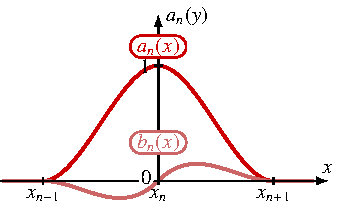
\includegraphics[scale=0.95,valign=t]{papers/fem/images/kubisch_formfkt.pdf}
        \label{fem:1d:abb:kubisch:formfkt}
    }
    
    \subfloat[Skalierte Formfunktionen mit der zu interpolierenden Funktion $f(x)$]{
        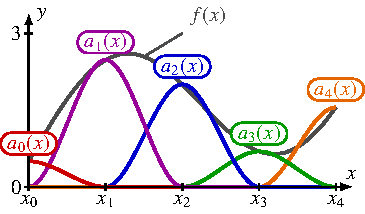
\includegraphics[scale=0.95,valign=t]{papers/fem/images/kubisch_formfkt_skaliert.pdf}
        \hfill
        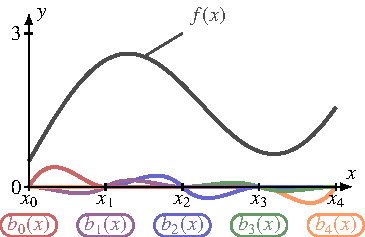
\includegraphics[scale=0.95,valign=t]{papers/fem/images/kubisch_formfkt_skaliert_diff}
        \label{fem:1d:abb:kubisch:skaliert}
    }

    \subfloat[Gegenüberstellung der interpolierten und der ursprünglichen Funktion.]{
        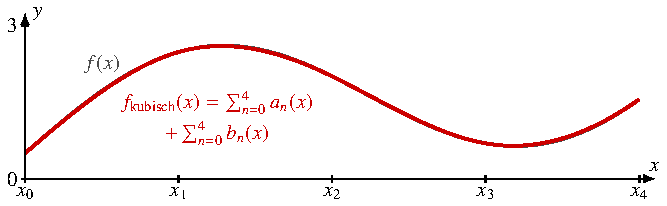
\includegraphics[scale=0.95,valign=t]{papers/fem/images/kubisch_interpoliert.pdf}
        \label{fem:1d:abb:kubisch:vergleich}
    }
    \caption{Kubische Interpolation des Signals $f(x)$.}
    \label{fem:1d:abb:kubisch}
\end{figure}
    